\section{The helium-3 shell flash: a provisional result}\label{sec:flash}

\subsection{Boundary condition and ignition}
Track S ends at $4.002\Tyr$ because its TLUSTY atmosphere families stop
at $\log g=6.1$. To continue, the outer boundary was replaced at that point
by the pure-hydrogen white-dwarf table distributed with MESA
\cite{rohrmann11,mesa_atm}, joined at optical depth 25.12, with the interior
composition and all evolution checks retained. The two prescriptions are not
equivalent: at 4600 K and $\log g=5.9$ the table gives a joining temperature
2.594\% higher and a gas pressure 48.69\% lower than an independently
converged TLUSTY atmosphere, and neither trace helium, the joining depth
(sampled between optical depth 168 and 4775) nor the atmosphere convection
prescription (ML2 with $\alpha=0.6$ and 1.0 change the joining values by
at most 0.04571\% and 0.2736\%) removes the difference. The continuation is
therefore a change of boundary condition, not a refinement.

Figure~\ref{fig:switch} shows the response. The surface temperature first
falls to 4362 K, the radius grows by 36.02\%, and after 0.7546 Gyr, at
$4.003\Tyr$ and 4632 K, the ratio of nuclear to photon luminosity has risen
to 2366: a helium-3 burning shell near $m/M=0.96$ has become convective.
The reaction $^3{\rm He}+{}^3{\rm He}\rightarrow{}^4{\rm He}+2p$ consumes the
accumulated helium-3 and returns hydrogen. Before the switch the shell was
fading, and every flash history computed so far descends from this one
post-switch state.

\begin{figure}[H]\centering
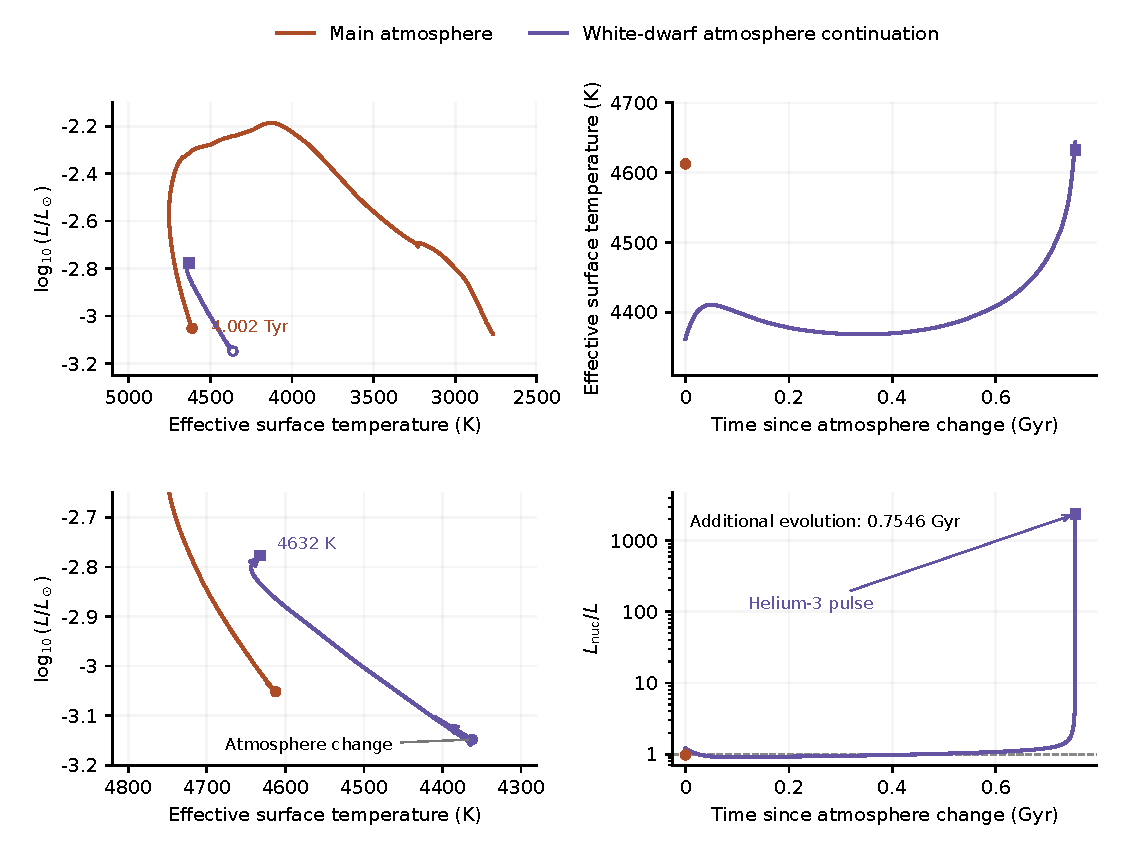
\includegraphics[width=\textwidth]{wd_atmosphere_response.pdf}
\caption{Track S with two atmosphere prescriptions. Orange: the TLUSTY
families through $4.002\Tyr$. Purple: the continuation with the
pure-hydrogen white-dwarf table, which differs from the TLUSTY boundary by
2.6\% in temperature and 49\% in pressure at the joining depth in the
sampled 4600 K, $\log g=5.9$ atmosphere, so the
initial offset is a change of boundary condition. Left: the HR track and an
enlarged view of the adjustment. Right: surface temperature and the ratio of
nuclear to photon luminosity against time since the switch (logarithmic
scale below). The continuation covers 0.7546 Gyr in 252 accepted intervals
and ends as a helium-3 shell becomes convective.}
\label{fig:switch}
\end{figure}

\subsection{What is established}
The pulse forms on every mass grid tried (578, 666, 848, 1695, 1763, 1899,
1923, 1983, 2010 and 2115 points, all refined around the burning layer) and
with both instantaneous and finite convective mixing. Nuclear power rises
from a quiescent $3\times10^{30}$ erg s$^{-1}$ to $1$--$2\times10^{36}$
erg s$^{-1}$ while the photon luminosity stays near $7\times10^{30}$ erg
s$^{-1}$: the released energy goes into the structure. Hydrostatic evolution
remains valid; at the coarse-grid endpoint the local heating time
$c_PT/\epsilon_{\rm nuc}$ is 472.4 yr against a dynamical time of 23.46 s.
The shell is only partly degenerate. Before shell convection the most
productive cell, at $m/M=0.9612$ and 10.72 MK, has thermal expansion
coefficient $\delta=0.9099$, close to the ideal-gas value, a logarithmic
temperature sensitivity of the heating rate of 16.52, and a thickness
0.05541 times its radius; thin-shell geometry and strong temperature
sensitivity support a thermal instability without strong degeneracy. The
same mechanism has been found in slowly accreting white dwarfs, where
helium-3 from incomplete pp burning ignites a convective layer before a nova
outburst \cite{denissenkov13}; the fuel supply and structure differ, so the
precedent supports the mechanism, not the amplitude.

Through 3422 yr on the 666-point grid the accepted nuclear powers integrate
to $7.964\times10^{45}$ erg, about 5\% of the $1.561\times10^{47}$ erg that
burning the whole helium-3 inventory would release; surface radiation
carries about $7\times10^{41}$ erg over the same interval. Nuclear energy
plus escaping neutrinos agrees with the change in nuclear rest mass. During
the pulse the first-law residual is measured against the larger of nuclear
and photon luminosity, with a relative limit of $2\times10^{-8}$.

\subsection{What is not established}
\emph{Spatial convergence.} Table~\ref{tab:grids} and
Figure~\ref{fig:grids} show that the amplitude and timing of the burning are
not converged. At equal remaining helium-3, the finite-mixing calculations on
578 and 666 points differ in nuclear power by a factor of 2.901; over a
matched 100 yr on 1927 and 1983 points the deposited energy differs by
8.261\% and the final power by 15.24\%; subdividing the burning layer
fourfold (1695 to 1923 points) over 688.5 yr reduces the deposited energy by
55.17\%. Later, during the decline, successive refinements agree to
0.5--1.5\%, which supports the shell-burning phase but not the onset or the
peak. Inserting mass points causes a mechanical readjustment with an initial
energy residual of $1.844\times10^{43}$ erg, identified as geometric rather
than physical. Convective regions that grow across the composition gradient
merge abruptly (near 3006 and 3341 yr on the finest grids), and substep
tests across the mergers agree to 0.01--0.3\% in integrated energy while a
gradual-mixing variant differs by 10.17\%; the internal timing of each
merger is unresolved.

\begin{table}[H]\centering\small
\caption{Flash calculations from the common post-switch model. Time is
measured from the common profile before shell convection; ``peak'' means the
largest value reached, not a converged maximum.}\label{tab:grids}
\begin{tabular}{@{}lp{0.3\textwidth}lrr@{}}\toprule
Points & Mixing & Interval & Peak $L_{\rm nuc}$ (erg s$^{-1}$) & Max $T$ (MK) \\\midrule
578 & instantaneous / finite & 1647 yr & --- & 15.30 \\
666 & instantaneous / finite & 2139 yr & $2.671\times10^{35}$ & 15.29 \\
666 & finite, energy flux on cell faces & 3429 yr & $5.537\times10^{36}$ & 21.86 \\
848 & finite, energy flux on cell faces & 3342 yr & $4.835\times10^{36}$ & 21.73 \\
1695 & finite, energy flux on cell faces & 6803 yr & $3.281\times10^{35}$ & 15.39 \\
1983 (F1) & finite from onset, all convective layers & 5.744 Myr & --- & --- \\
2115 (F2) & instantaneous then finite & 42.48 Myr & --- & --- \\\bottomrule
\end{tabular}
\end{table}

\begin{figure}[H]\centering
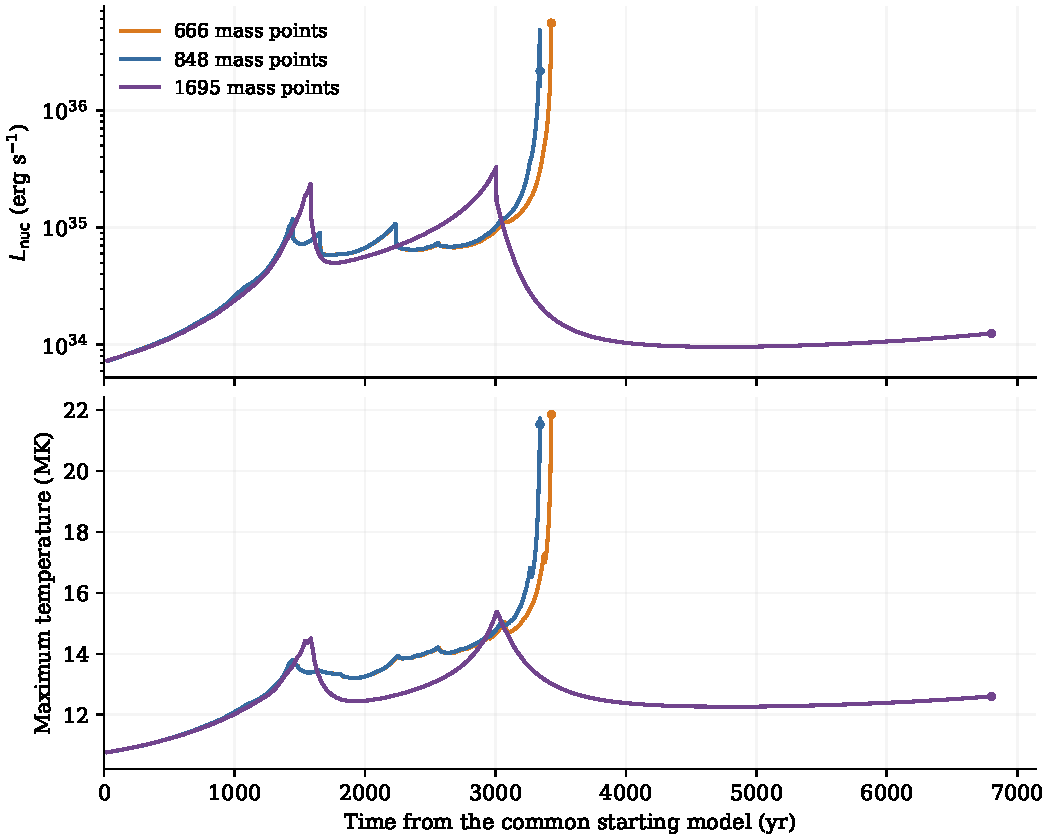
\includegraphics[width=0.92\textwidth]{pulse_face_comparison.pdf}
\caption{Nuclear luminosity and maximum internal temperature on three mass
grids, with total energy and composition enthalpy transported across the
same mass surfaces. All use the white-dwarf table boundary and finite
convective mixing without semiconvection; time runs from the common profile
before shell convection. The largest sampled shell temperatures are
21.86, 21.73 and 15.39 MK; the finest grid reaches 12.60 MK
after a long decline and modest reheating. Sharp decreases near 3006 and
3341 yr are convective-region mergers. Their largest sampled nuclear powers
differ by more than an order of magnitude; the peak is not converged.}
\label{fig:grids}
\end{figure}

\emph{Dependence on the boundary prescription.} Both flash continuations
inherit the white-dwarf table's normalization, which differs from the
TLUSTY boundary by 2.6--3.0\% in temperature and 49--91\% in pressure at the
states sampled. Applying the calculated mixed-to-hydrogen composition ratios
to the hydrogen table retains that normalization rather than testing it.
Comparisons of two extrapolations of the table below $\log g=5.5$, over
$10^3$--$2\times10^6$ yr, change the endpoint temperature by at most
11.27 K and the deposited nuclear energy by at most 0.03\%; these test the
extension, not the absolute boundary. The pulse develops 0.7546 Gyr after
the switch, but that delay does not show that it is independent of the
switch: the shell was fading before it, and the LBA97 model, the grey MESA
sequences and Ember's own grey-boundary sequence (Section~\ref{sec:mesa})
show no flash. Whether ignition survives the original atmosphere can be
decided only by a comparison that starts before the histories diverge. A
pure-hydrogen TLUSTY source rectangle at optical depth 100 above
$\log g=5.95$ is being computed for that control; the 4800 K, $\log g=6.0$
columns are already validated, and the control is pending.

\emph{Mixing physics.} The flash calculations set semiconvective and
thermohaline coefficients to zero. The reaction that powers the flash lowers
the mean molecular weight and can drive thermohaline mixing, as in red
giants \cite{charbonnel07}; whether it does so strongly enough to alter the
shell requires the composition gradient and transport times to be assessed.
Holding the mixing coefficient at its beginning-of-step value during each
implicit solve, as MESA does \cite{paxton11}, passes the species and energy
checks with successive changes of 0.09470\%, 0.04722\% and 0.02357\% in
integrated nuclear energy, but pointwise composition differences do not
decrease.

\subsection{The two continuations}
Two histories were carried through the pulse from the same post-switch
model (Figure~\ref{fig:histories}, Table~\ref{tab:histories}). F1 applies
finite composition transport throughout all convective layers from the onset
of shell convection. F2 first mixes the cooler convective layers
instantaneously, then uses finite transport once the shell convection
connects to the surface envelope; its accumulated thermal and composition
history therefore differs from F1's, and local checks of its later evolution
do not establish that it is F1's outcome. In F2 the envelope becomes
helium-enriched when the convective regions connect: over a checked 0.6656 yr
the surface hydrogen falls from 0.9984 to 0.8085 while helium-3 rises to
0.007264, yet 99\% of the metals remain inside $m/M=0.4456$, so the
atmosphere can be helium-rich while remaining nearly metal-free. Both
histories pass a radius maximum before their temperature maximum: expansion
is followed by contraction during which the surface heats while the
luminosity falls, consistent with delayed structural adjustment. At their
endpoints both are declining in temperature but remain 33--56\%
nuclear-powered, with most of the remaining helium-3 outside the burning
layer. In F2 at $1.345\times10^4$ yr the outer convective envelope, then
4.033\% of the mass, holds 86.44\% of the remaining helium-3 but supplies
0.7504\% of the nuclear power; between $1.443\times10^4$ and
$1.701\times10^4$ yr it loses only 0.01453\% of its helium-3 while the
active layers deplete. The fuel that could power a later episode is
therefore separated from the burning region, and its consumption depends on
transport that these calculations do not yet resolve; fuel depletion alone
does not exclude another unstable episode, and neither history is a
white-dwarf cooling sequence.

\begin{table}[H]\centering\small
\caption{Endpoints of the two flash continuations. Times from the common
model before shell convection; both provisional.}\label{tab:histories}
\begin{tabular}{@{}lrr@{}}\toprule
 & F1 (1983 points) & F2 (2115 points) \\\midrule
Time computed & 5.744 Myr & 42.48 Myr \\
Saved $\Teff$ maximum & 6422 K at 1.139 Myr & 6399 K at 1.088 Myr \\
Endpoint $\Teff$ & 5903 K & 4771 K \\
Endpoint nuclear power (erg s$^{-1}$) & $1.126\times10^{31}$ & $3.166\times10^{30}$ \\
Nuclear share of surface luminosity & 32.84\% & 55.85\% \\
Endpoint radius & $0.09048\Rs$ & $0.05633\Rs$ \\
Surface $X$, $X_3$ & --- & 0.8200, 0.007167 \\
Remaining hydrogen & --- & $0.003792\Ms$ \\
Central $T$, $\rho$ & --- & 6.192 MK, $3.932\times10^4$ g cm$^{-3}$ \\\bottomrule
\end{tabular}
\end{table}

\begin{figure}[H]\centering
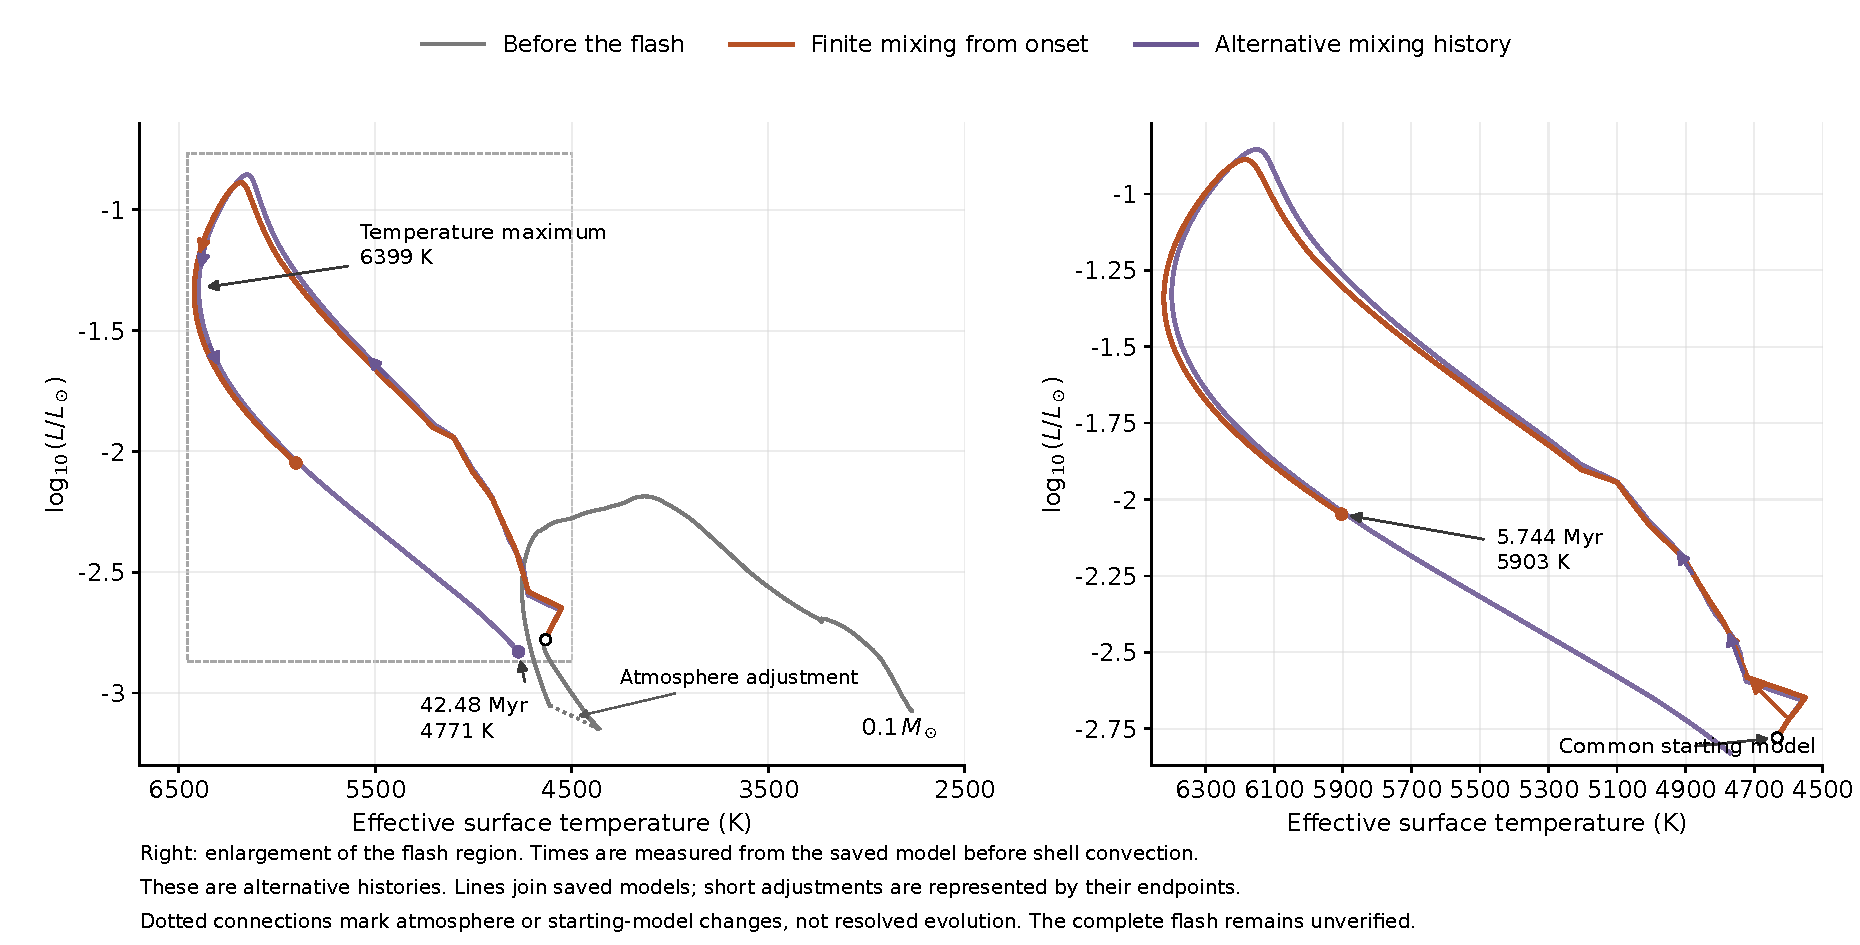
\includegraphics[width=0.95\textwidth]{flash_histories_hr.pdf}\\[4pt]
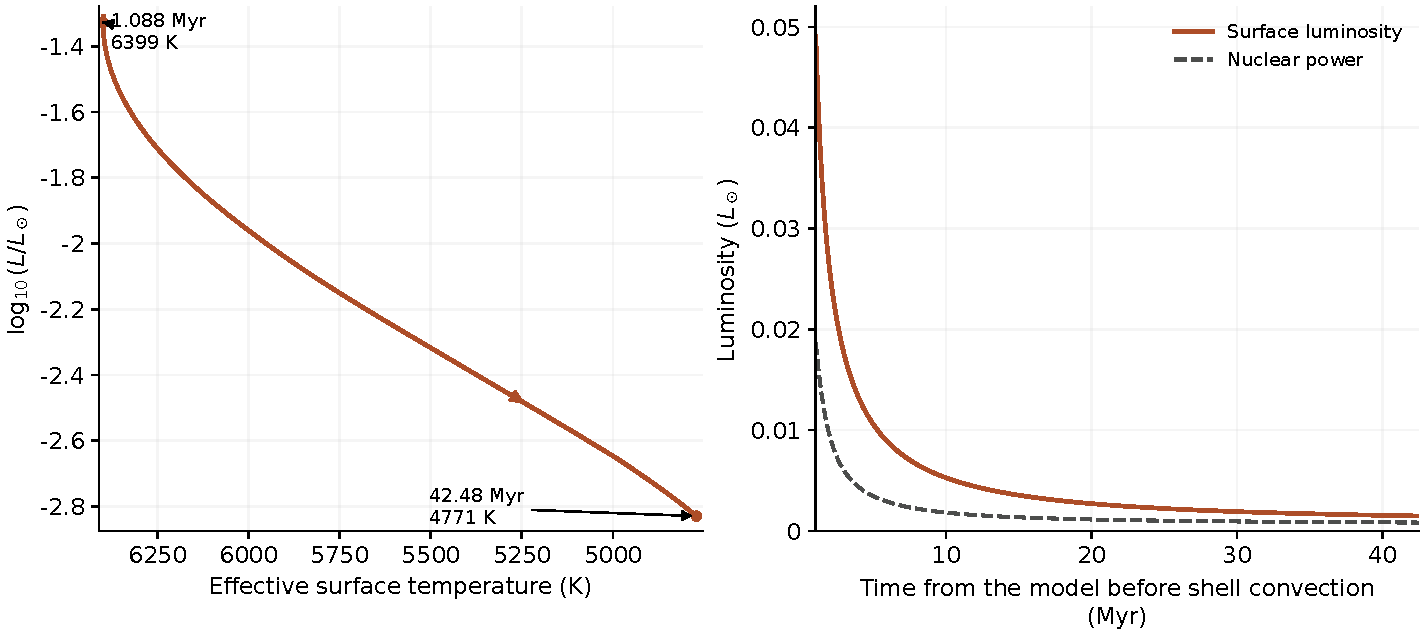
\includegraphics[width=0.95\textwidth]{late_cooling.pdf}
\caption{The two flash continuations. Upper: HR tracks of F1 (orange,
finite mixing from onset) and F2 (purple, alternative mixing history), with
the preceding Track S evolution in gray; dotted connections mark the
atmosphere switch and starting-model adjustments, not resolved evolution.
The right panel enlarges the flash region. Lower: F2 on 2115 points, an
enlarged HR diagram around its temperature maximum (left) and photon
luminosity with deposited nuclear power against time (right). Both
histories use the white-dwarf table boundary switched in at $4.002\Tyr$;
whether the flash occurs with the original atmosphere has not been tested.
Agreement of the two HR tracks does not establish convergence of the peak
power or of the internal mixing.}
\label{fig:histories}
\end{figure}

At 29.48 Myr in F2 the reduced pp network produces helium-3 at
$1.263\times10^{12}$ g s$^{-1}$ and destroys it at $4.106\times10^{11}$
g s$^{-1}$, and helium-3 fusion supplies 23.12\% of the nuclear power,
down from 26.97\% five million years earlier; summing the saved sources
reproduces the inventory change to better than $10^{-10}$. This
establishes the production--destruction balance, not stability against a
later flash. In F2 at 12.07 Myr, 46.16\% of the nuclear power comes from
$^3$He+$^3$He, 49.94\% from the hydrogen reactions that build $^3$He and
3.901\% from the reduced ppII branch; the helium-3 inventory is 82.97\% of
its value in the common starting model. Between $2.012\times10^5$ and
$2.512\times10^5$ yr, nuclear burning supplies 31.97\% of the integrated
surface emission and structural adjustment 68.03\%. The atmosphere tables
entered by the continuations (hydrogen--helium mixtures at 4500--6500 K and
$\log g=4.2$--5.8) were checked for depth and interpolation to better than
0.2\% in temperature and 1.1\% in pressure (Appendix~\ref{app:tech}); the
absolute hydrogen normalization remains the unresolved uncertainty.
